\chapter{Исследовательская часть}

\section{Технические характеристики}

Технические характеристики устройства, на котором выполнялось тестирование представлены далее.

\begin{itemize}
	\item Процессор: Intel(R) Core(TM) i5-10300H CPU @ 2.50 GHz 2.50 GHz.
	\item Оперативная память: 16 GiB.
	\item Операционная система: Windows 10 Pro 21H2 64-bit.
\end{itemize}

При тестировании ноутбук был включен в сеть электропитания. Во время тестирования ноутбук был нагружен только встроенными приложениями
окружения, а также системой тестирования.

\section{Демонстрация работы программы}

\begin{figure}[h]
	\centering
	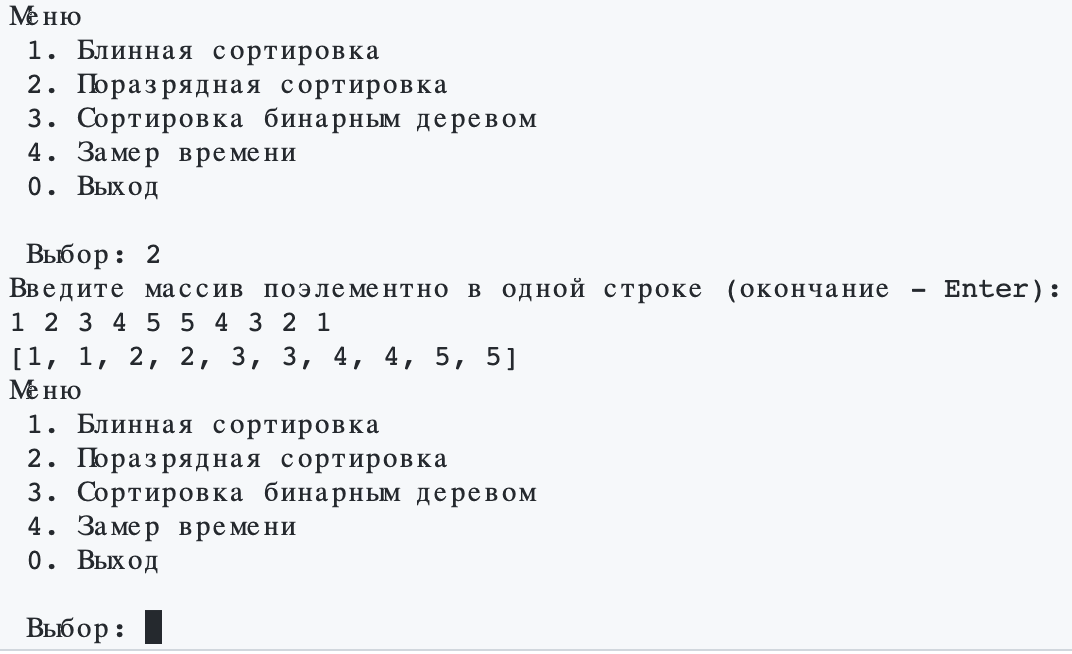
\includegraphics[height=0.4\textheight]{img/example.png}
	\caption{Демонстрация работы программы при поиске расстояние Левенштейна и Дамерау-Левенштейна}
	\label{img:demonstration}
\end{figure}

\clearpage

\section{Временные характеристики}

Результаты замеров по результатам экспериментов приведены в Таблице \ref{tbl:time}. В данной таблице для значений, для которых тестирование не выполнялось, в поле результата находится "\ - ".

\begin{table}[ht]
	\small
	\begin{center}
		\caption{Замер времени для строк, размером от 1 до 200}
		\label{tbl:time}
		\begin{tabular}{|c|c|c|c|c|}
			\hline
			& \multicolumn{4}{c|}{\bfseries Время, нс} \\ \cline{2-5}
			& \multicolumn{1}{c|}{\bfseries Левенштейн}
			& \multicolumn{3}{c|}{\bfseries Дамерау-Левенштейн} \\ \cline{2-5}
			\bfseries Длина (символ) & \bfseries Итеративный & \bfseries Итеративный & \multicolumn{2}{c|}{\bfseries Рекурсивный} \\ \cline{4-5}
			& & & \bfseries Без кэша & \bfseries С кэшом
			\csvreader{csv/time.csv}{}
			{\\\hline \csvcoli & \csvcolii & \csvcoliii & \csvcoliv & \csvcolv} \\
			\hline
		\end{tabular}
	\end{center}
\end{table}

Отдельно сравним итеративные алгоритмы поиска расстояний Левенштейна и Дамерау--Левенштейна. Сравнение будет производится на основе данных, представленных в Таблице \ref{tbl:time}. Результат можно увидеть на Рисунке \ref{plt:time_01}.

При длинах строк менее 30 символов разница по времени между
итеративными реализациями незначительна, однако при увеличении длины
строки алгоритм поиска расстояния Левенштейна оказывается быстрее
вплоть до полутора раз (при длинах строк равных 200). Это обосновывается
тем, что у алгоритма поиска расстояния Дамерау-Левенштейна задействуется
дополнительная операция, которая замедляет алгоритм

\begin{figure}[h]
	\centering
	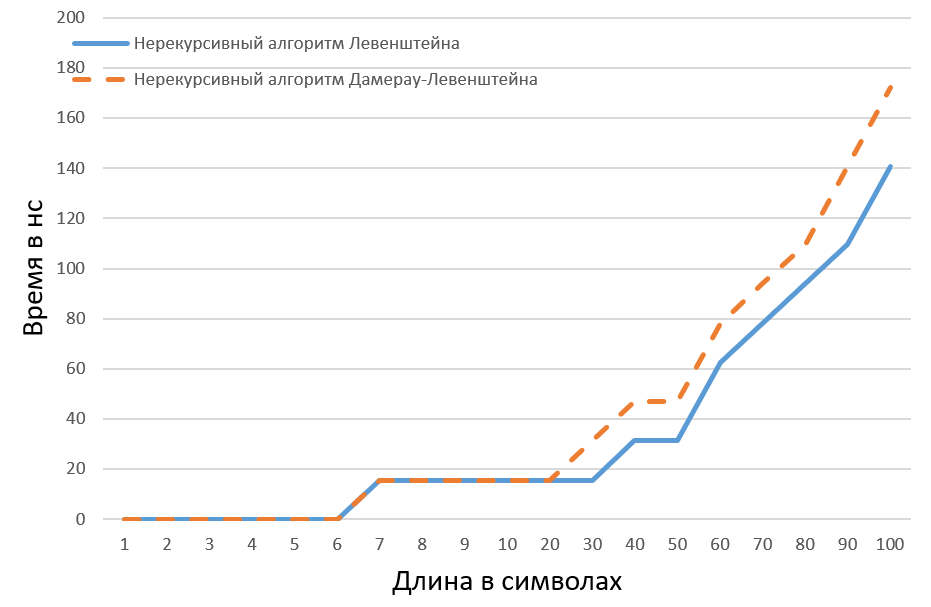
\includegraphics[height=0.3\textheight]{img/diag_01.png}
	\caption{Сравнение по времени алгоритмов поиска расстояния Левенштейн и Дамерау-Левенштейна -- нерекурсивной реализации}
	\label{plt:time_01}
\end{figure}

Так же сравним рекурсивную и итеративную реализации алгоритма поиска расстояния Дамерау-Левенштейна. Данные представлены в Таблице \ref{tbl:time} и отображены на Рисунке \ref{plt:time_02}.

\begin{figure}[h]
	\centering
	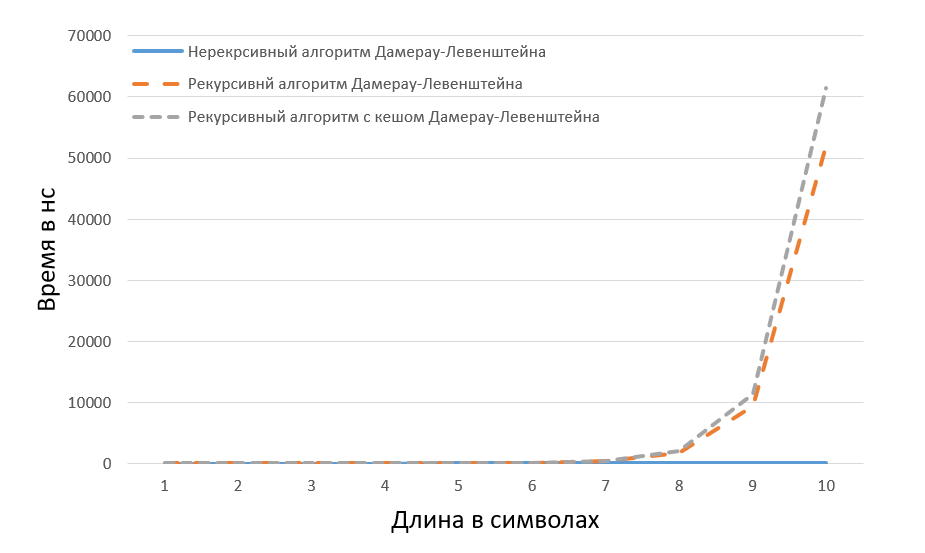
\includegraphics[height=0.3\textheight]{img/diag_02.png}
	\caption{Сравнение по времени алгоритмов поиска расстояния Дамерау-Левенштейна}
	\label{plt:time_02}
\end{figure}

На Рисунке \ref{plt:time_02} продемонстрировано, что рекурсивный алгоритм становится менее эффективным (вплоть до 21 раз при длине строк равной 7 элементов), чем итеративный.

Из этого можно сделать вывод о том, что при малых длинах строк (1-4 символа) предпочтительнее использовать рекурсивные алгоритмы, однако при обработке более длинных строк (болеее 3 символов) итеративные алгоритмы оказываются многократно более эффективными и рекомендованы к использованию.

Из данных, приведенных в  Таблице \ref{tbl:time}, видно, что итеративные алгоритмы становятся более эффективными по времени при увеличении длин строк, работая приблизительно в 308 млн. раз (Левенштейн) и 203 млн. раз (Дамерау-Левенштейн) быстрее, чем рекурсивные (при длинах строк равных 200). Однако, при малых длинах (1-4 элемента) рекурсивные алгоритмы работает по примерно как итеративные.

Кроме того, согласно данным, приведенным в Таблице \ref{tbl:time}, рекурсивные алгоритмы при длинах строк более 10 элементов не пригодны к использованию в силу экспоненциально роста затрат процессорного времени, в то время, как затраты итеративных алгоритмов по времени линейны.

\section{Характеристики по памяти}

Введем следующие обозначения:
\begin{itemize}
	\item$n$ - длина строки $S_{1}$;
	\item$m$ - длина строки $S_{2}$;
	\item$size()$ - функция вычисляющая размер в байтах;
	\item $string$ - строковый тип;
	\item $int$ - целочисленный тип;
	\item $size\_t$ - беззнаковый целочисленный тип.
\end{itemize}

Максимальная глубина стека вызовов при рекурсивной реализации нахождения расстояния Дамерау-Левенштейна равна сумме входящих строк, а на каждый вызов требуется 4 дополнительных переменных, соответственно, максимальный расход памяти.
\begin{equation}
	(n + m) \cdot (2 \cdot size(string) + 3 \cdot size(int) + 2 \cdot sizeof(size\_t))
\end{equation}
, где:
\begin{itemize}
	\item хранение двух строк - $2 \cdot size(string)$;
	\item хранение размеров строк - $2 \cdot size(size\_t)$;
	\item дополнительные переменные - $2 \cdot size(int)$;
	\item адрес возврата.
\end{itemize}

Для рекурсивного алгоритма Дамерау-Левенштейна будет теоретически тоже самое, что и в рекурсивном, но добавляется еще размер матрицы, соответственно, максимальный расход памяти:
\begin{equation}
	(n + m) \cdot (2 \cdot size(string) + 3 \cdot size(int) + 2 \cdot size(size\_t)) + (n + 1) \cdot (m + 1) \cdot size(int)
\end{equation}

Использование памяти при итеративной реализации расстояния Левенштейна теоретически равно сумме всех перечисленных элементов:
\begin{itemize}
	\item хранение двух строк - $2 \cdot size(string)$;
	\item хранение размеров матрицы - $2 \cdot size(size\_t)$;
	\item хранение матрицы - $(n + 1) \cdot (m + 1) \cdot ыize(int)$;
	\item указатель на матрицу - $size(int **) + (n + 1) \cdot size(int *)$;
	\item дополнительные переменные для хранения результата - $size(int)$;
	\item адрес возврата.
\end{itemize}

Использование памяти при итеративной реализации расстояния Дамерау-Левенштейна теоретически равно сумме всех перечисленных элементов:
\begin{itemize}
	\item хранение двух строк - $2 * size(string)$;
	\item хранение размеров матрицы - $2 \cdot size(size\_t)$;
	\item хранение матрицы - $(n + 1) \cdot (m + 1) \cdot size(int)$;
	\item указатель на матрицу - $size(int **) + (n + 1) \cdot size(int *)$;
	\item дополнительные переменные - $2 \cdot size(int)$;
	\item адрес возврата.
\end{itemize}

По расходу памяти итеративные алгоритмы проигрывают рекурсивным: максимальный размер используемой памяти в них растет как произведение длин строк, в то время как у рекурсивного алгоритма — как сумма длин строк.

\begin{table}[ht]
	\small
	\begin{center}
		\caption{Замер памяти для строк, размером от 10 до 200}
		\label{tbl:memory}
		\begin{tabular}{|c|c|c|c|c|}
			\hline
			& \multicolumn{4}{c|}{\bfseries Размер в байтах} \\ \cline{2-5}
			& \multicolumn{1}{c|}{\bfseries Левенштейн}
			& \multicolumn{3}{c|}{\bfseries Дамерау-Левенштейн} \\ \cline{2-5}
			\bfseries Длина (символ) & \bfseries Итеративный & \bfseries Итеративный & \multicolumn{2}{c|}{\bfseries Рекурсивный} \\ \cline{4-5}
			& & & \bfseries Без кэша & \bfseries С кэшом
			\csvreader{csv/memory.csv}{}
			{\\\hline \csvcoli & \csvcolii & \csvcoliii & \csvcoliv & \csvcolv} \\
			\hline
		\end{tabular}
	\end{center}
\end{table}

Из данных, приведенных в Таблице \ref{tbl:memory}, видно, что рекурсивные алгоритмы являются более эффективными по памяти, так как используется только память под локальные переменные, передаваемые аргументы и возвращаемое значение, в то время как итеративные алгоритмы затрачивают память линейно пропорционально длинам обрабатываемых строк.

В связи с этим, при недостаточном объеме памяти, рекомендуются использовать рекурсивные алгоритмы, так как они не используют дополнительной памяти в процессе работы.

\clearpage

\begin{figure}[h]
	\centering
	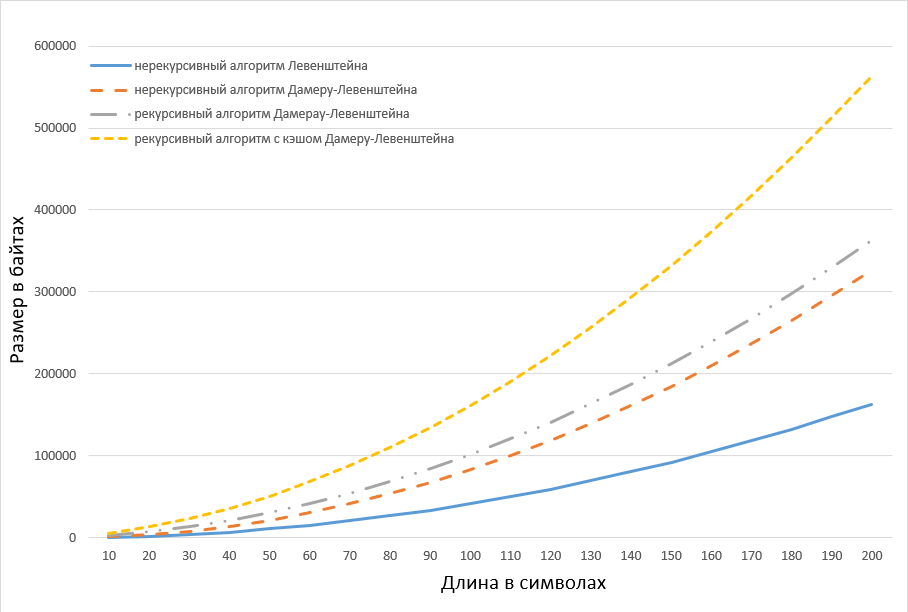
\includegraphics[height=0.3\textheight]{img/diag_03.png}
	\caption{Сравнение по памяти алгоритмов поиска расстояния Левенштейна и Дамерау-Левенштейна -- итеративной и рекурсивной реализации}
	\label{plt:memory}
\end{figure}

\section{Сравнительный анализ алгоритмов}
Приведенные характеристики показывают нам, что рекурсивная реализация алгоритма очень сильно проигрывает по времени. В связи с этим, рекурсивные алгоритмы следует использовать лишь для малых размерностей строк (1-4 символа) или при малом объеме оперативной памяти.

Так как во время печати очень часто возникают ошибки связанные с транспозицией букв, алгоритм поиска расстояния Дамерау-Левенштейна является наиболее предпочтительным, не смотря на то, что он проигрывает по времени и памяти алгоритму Левенштейна.

Можно сделать вывод о том, что рекуррентный алгоритм поиска расстояния Дамерау-Левенштейна будет более затратным по времени по сравнению с итеративной реализацией алгоритма поиска расстояния Дамерау-Левенштейна.

\section{Вывод}
В данном разделе было произведено сравнение количества затраченного времени и памяти вышеизложенных алгоритмов. Наименее затратным по времени оказался рекурсивный алгоритм нахождения расстояния Дамерау-Левенштейна.

Для обработок малых длин строк (1-4 символа) предпочтительнее использовать рекурсивные алгоритмы, в то время как для остальных случаев рекомендуются использовать итеративные реализации. Однако, стоит учитывать дополнительные затраты по памяти, возникающие при использовании итеративных алгоритмов.